\documentclass[11pt]{article}

\usepackage{amsmath}
\usepackage{textcomp}
\usepackage[top=0.8in, bottom=0.8in, left=0.8in, right=0.8in]{geometry}
% Add other packages here %
\usepackage{graphicx} 
\usepackage{booktabs}
\usepackage{float}



% Put your group number and names in the author field %
\title{\bf Exercise 1.\\ Implementing a first Application in RePast: A Rabbits Grass Simulation.}
\author{Group \textnumero24: Quentin Juppet, Andrea Piccione}

\begin{document}
\maketitle

\section{Implementation}

\subsection{Assumptions}
% Describe the assumptions of your world model and implementation (e.g. is the grass amount bounded in each cell) %
It was assumed that the grass is only spread on cells that are not occupied by other grass yet, so one cell has always one grass unit (amount of grass per cell bounded to 1). Furthermore, rabbits are not allowed to move if the random cell chosen for the simulation step is already occupied by another rabbit. 

Some additional parameters have been introduced in order to allow a more fine-grained control of the simulation:

- a StarvingEnergy parameter such that a rabbit can still lose a certain amount of energy (specified by the parameter) if it doesn't move: this is particularly useful when the space is completely filled by rabbits and it allows to make them die when they can't move anymore;

- a RabbitInitEnegy parameter to set the initial energy value of a rabbit at its creation; 

- a MoveEnergy parameter to specify the amount of energy lost by rabbits when they move;

- a EatGrassEnergy parameter to control the amount to energy gained by rabbits when they eat grass.


\subsection{Implementation Remarks}
% Provide important details about your implementation, such as handling of boundary conditions %
One important remark should be made about the scheduling of the events on each simulation step. As it can be seen from the buildSchedule() method in the RabbitsGrassSimulationModel class, all rabbits are first left to step and, only after each rabbit has stepped, it is checked if it possible to create new born rabbits in case the creation condition is fulfilled (it would have also been possible to spawn new rabbits inside each simulation step of a singular agent). Then, it is checked if some rabbits are dead (energy has reached 0) and finally new grass is spawn according to the GrassGrowthRate parameter. It might happen that new grass can spawn in a cell already occupied by a rabbit but this was considered a normal behavior.

We bounded the parameters to specific ranges. All the parameters can have a numeric value from 0 to 100, with the exception of GridSize and GrassGrowthRate which are in the range [0-50]. In general, all possible values are allowed but it is recommended to set them properly. 
% The only thing noticed was that a grid size equal to 0 makes the simulation crash.


\section{Results}
% In this section, you study and describe how different variables (e.g. birth threshold, grass growth rate etc.) or combinations of variables influence the results. Different experiments with different settings are described below with your observations and analysis


\subsection{Experiment 1}

\subsubsection{Setting}
Table 1 shows the main set of parameters used for this and the following experiments (additional variations will be reported in the appropriate sections). The MoveEnergy and StarvingEnergy parameters (both set to 1) have been omitted for simplicity because will not be extremely relevant for the following discussions. 

In this experiment, we analyze the evolution of the simulation with the standard parameters and we observe the importance of the introduced EatGrassEnergy parameter.

\begin{table}[h]
	\centering
	\caption{Default values for the experiments.}
    \begin{adjustbox}{\textwidth}
    \small
	\begin{tabular}{@{}lllllll{}@}
	    \hline
        BirthThreshold & EatGrassEnergy & GrassGrowthRate & RabbitInitEnergy & NumInitGrass & NumInitRabbits \\ 
        \hline
		75 & 20 & 10 & 50 & 25 & 5 \\
        \hline
	\end{tabular}
    \end{adjustbox}
\end{table}


\subsubsection{Observations}
% Elaborate on the observed results %
In the first phase of the simulation we notice that the amount of rabbits and grass start growing very quickly until we reach an equilibrium with approximately 90-100 rabbits and 50-60 grass units (Figure 1). This effect was expected since the grid is initially filled with a lot of grass and the few rabbits has the chance to get enough energy to reproduce. If we change the EatGrassEnergy value to 5 (Figure 2), we observe that an equilibrium is reached again but this time there are more grass units than rabbits because rabbits don't grow as much as before. We can see that for a certain range of acceptable values, by varying this parameter, it is possible to easily change the rabbit-grass ratio at the equilibrium in the long run.



\begin{figure}[h]
\centering
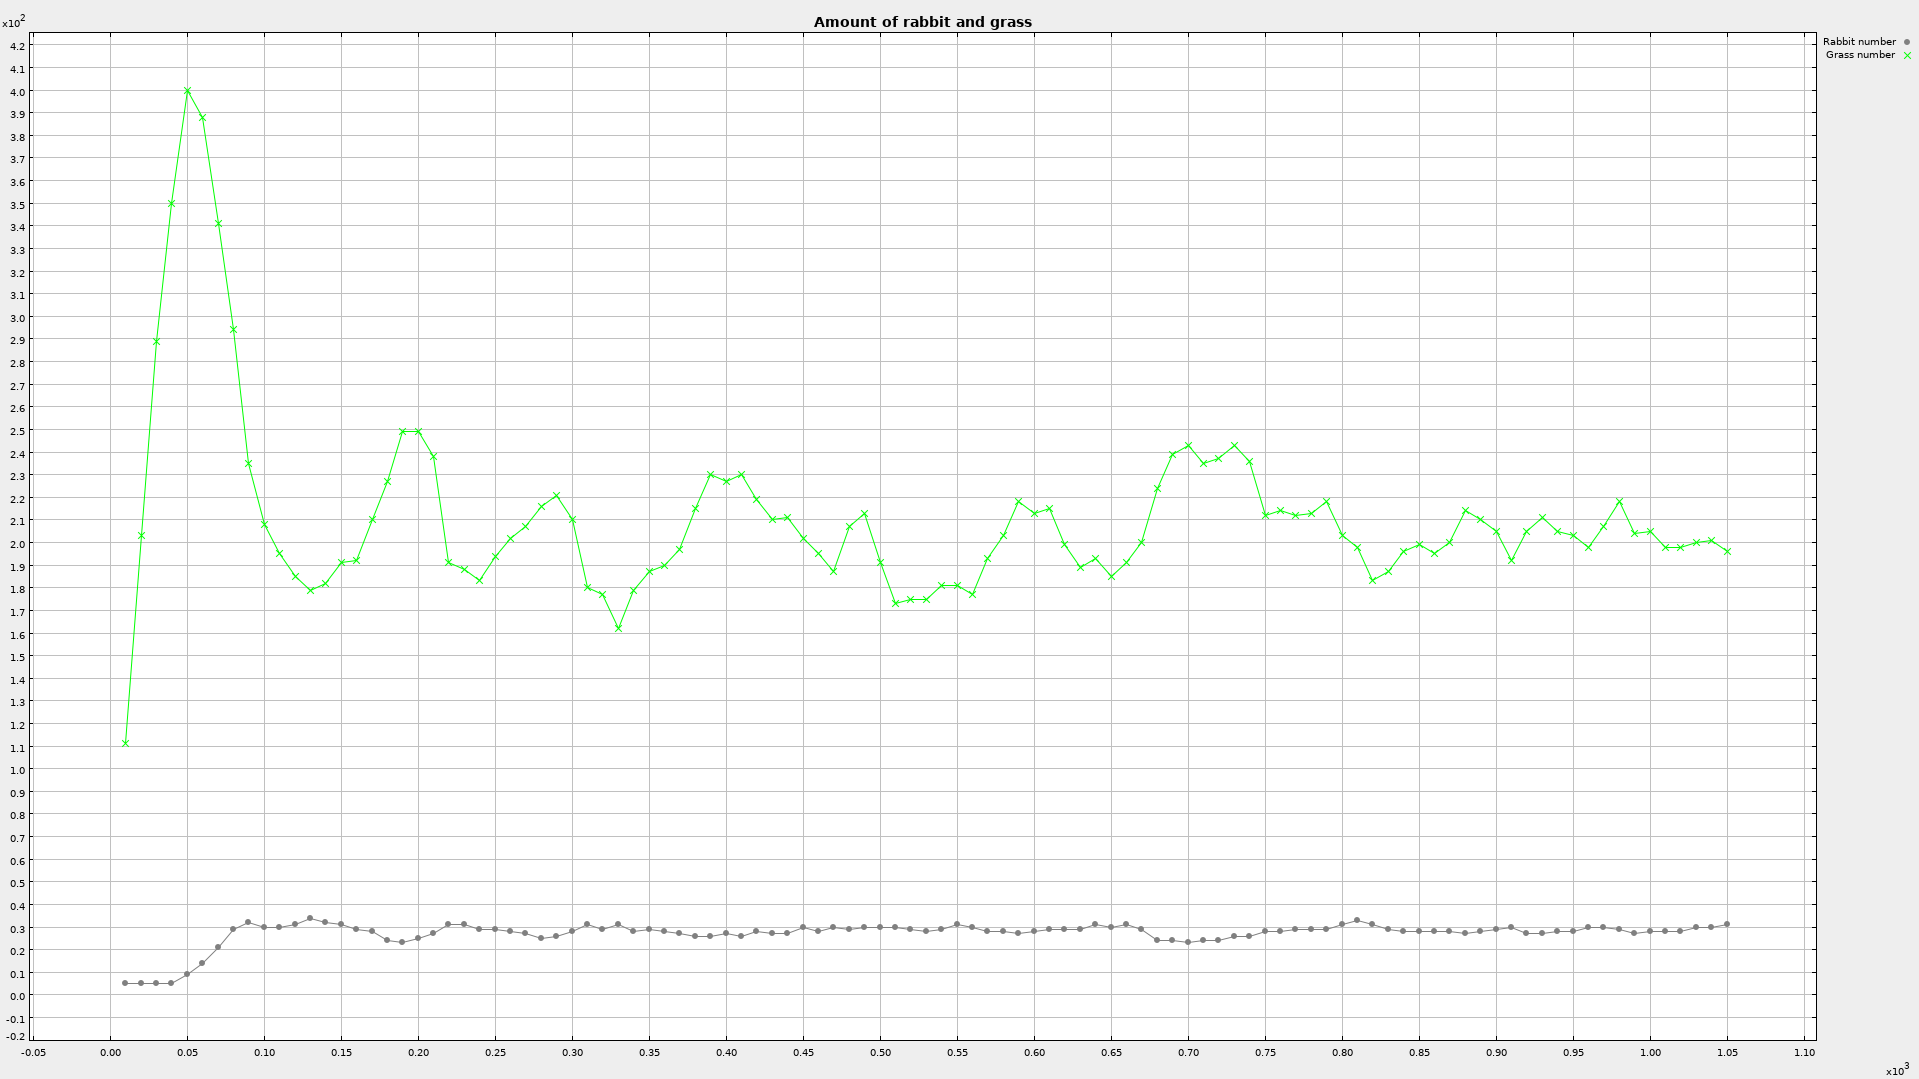
\includegraphics[width=1\linewidth, height=5cm]{setting1_1.png} 
\caption{Population plot for EatGrassEnergy = 20.}
\label{fig:subim1}
\end{figure}

\begin{figure}[h]
\centering
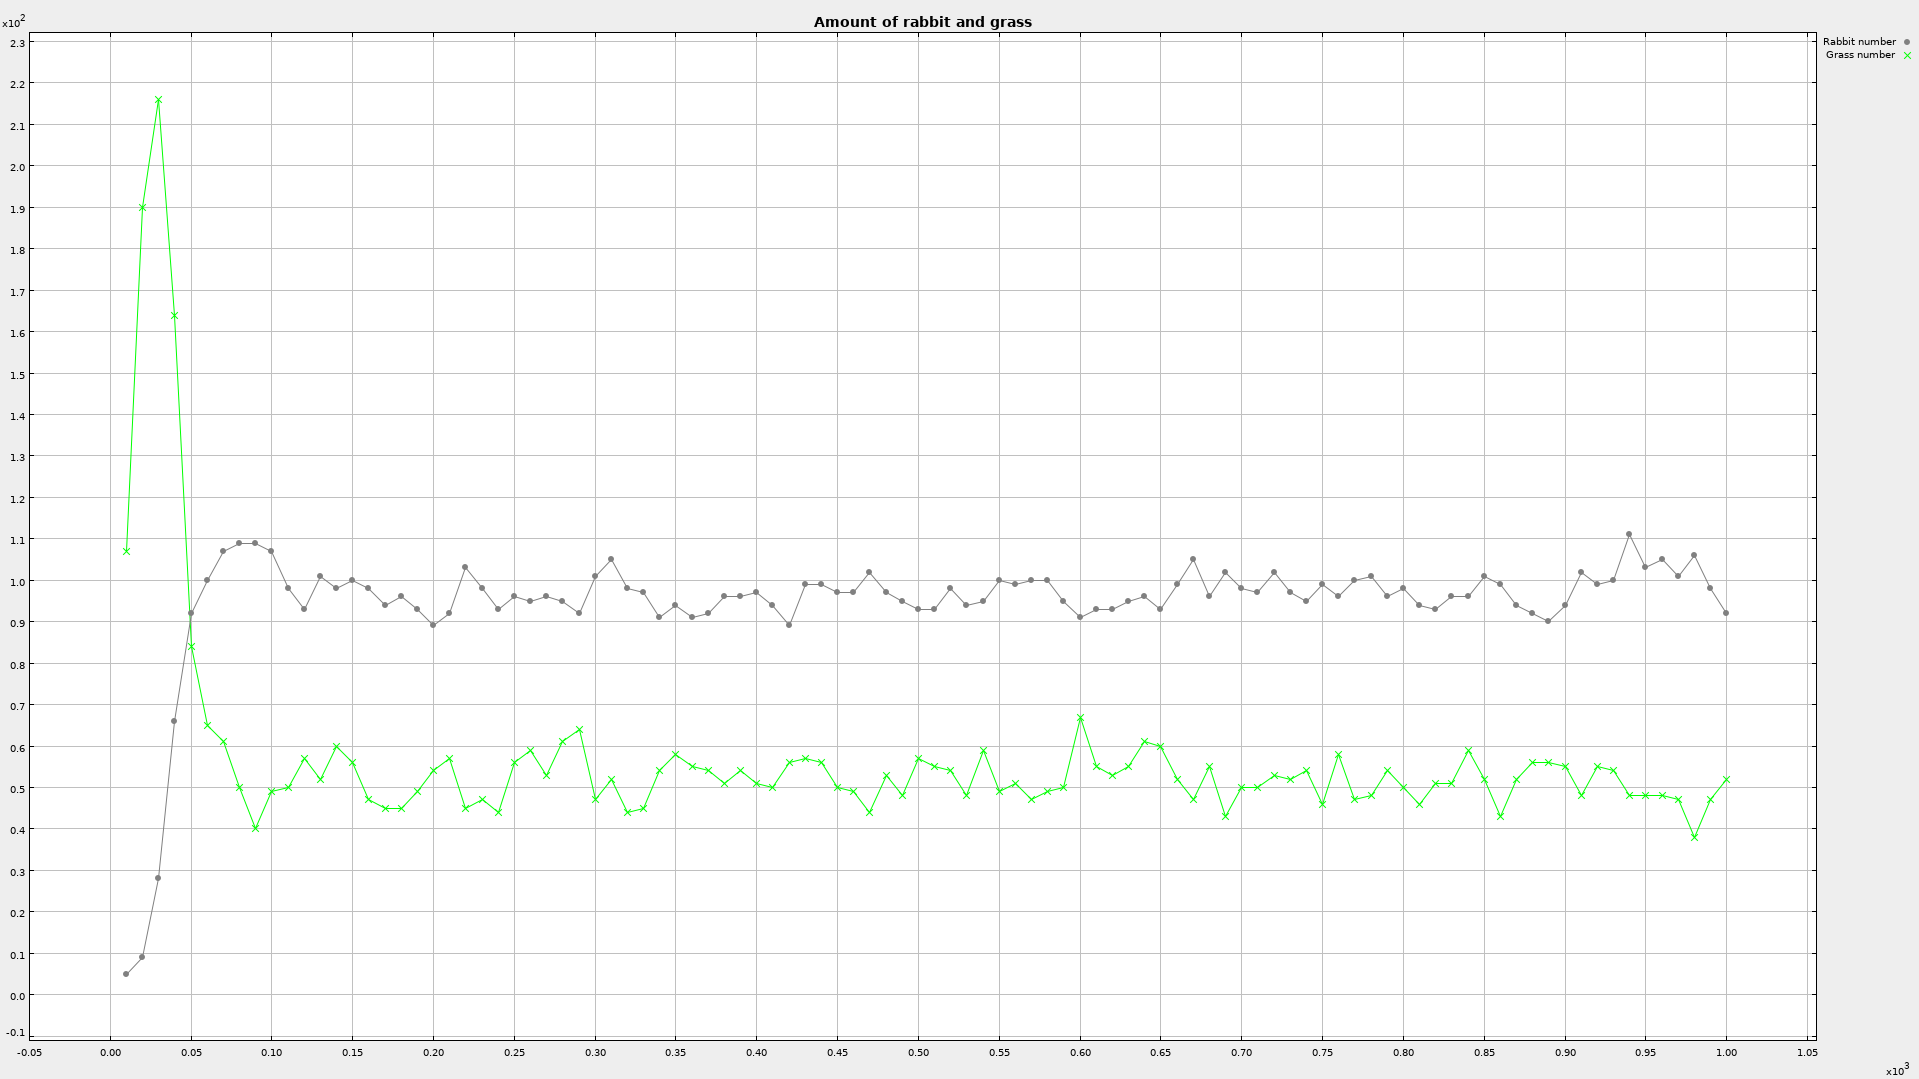
\includegraphics[width=1\linewidth, height=5cm]{setting2_2.png}
\caption{Population plot for EatGrassEnergy = 5.}
\label{fig:subim2}
\end{figure}


\subsection{Experiment 2}

\subsubsection{Setting}
We now take into consideration the GrassGrowthRate parameter and how this affects the simulation.

\subsubsection{Observations}
% Elaborate on the observed results %
For small values of GrassGrowthRate, it is clear how the number rabbits increases when the number of grass units decreases and vice versa, with lots of high and low peaks. This is similar to what it was observed in the previous experiment with EatGrassEnergy = 20 but in this case the equilibrium is less stable and more prone to fluctuations, especially for very small values. As shown in Figure 3, the extreme case where GrassGrowthRate = 1 shows initially a constant series of fluctuations until a divergent point where all rabbits are dead and the grid is completely filled with grass. For values higher than 10 the number of rabbits is usually very high and remains constant to a number close to 400 even after many steps.   


\begin{figure}[h]
\centering
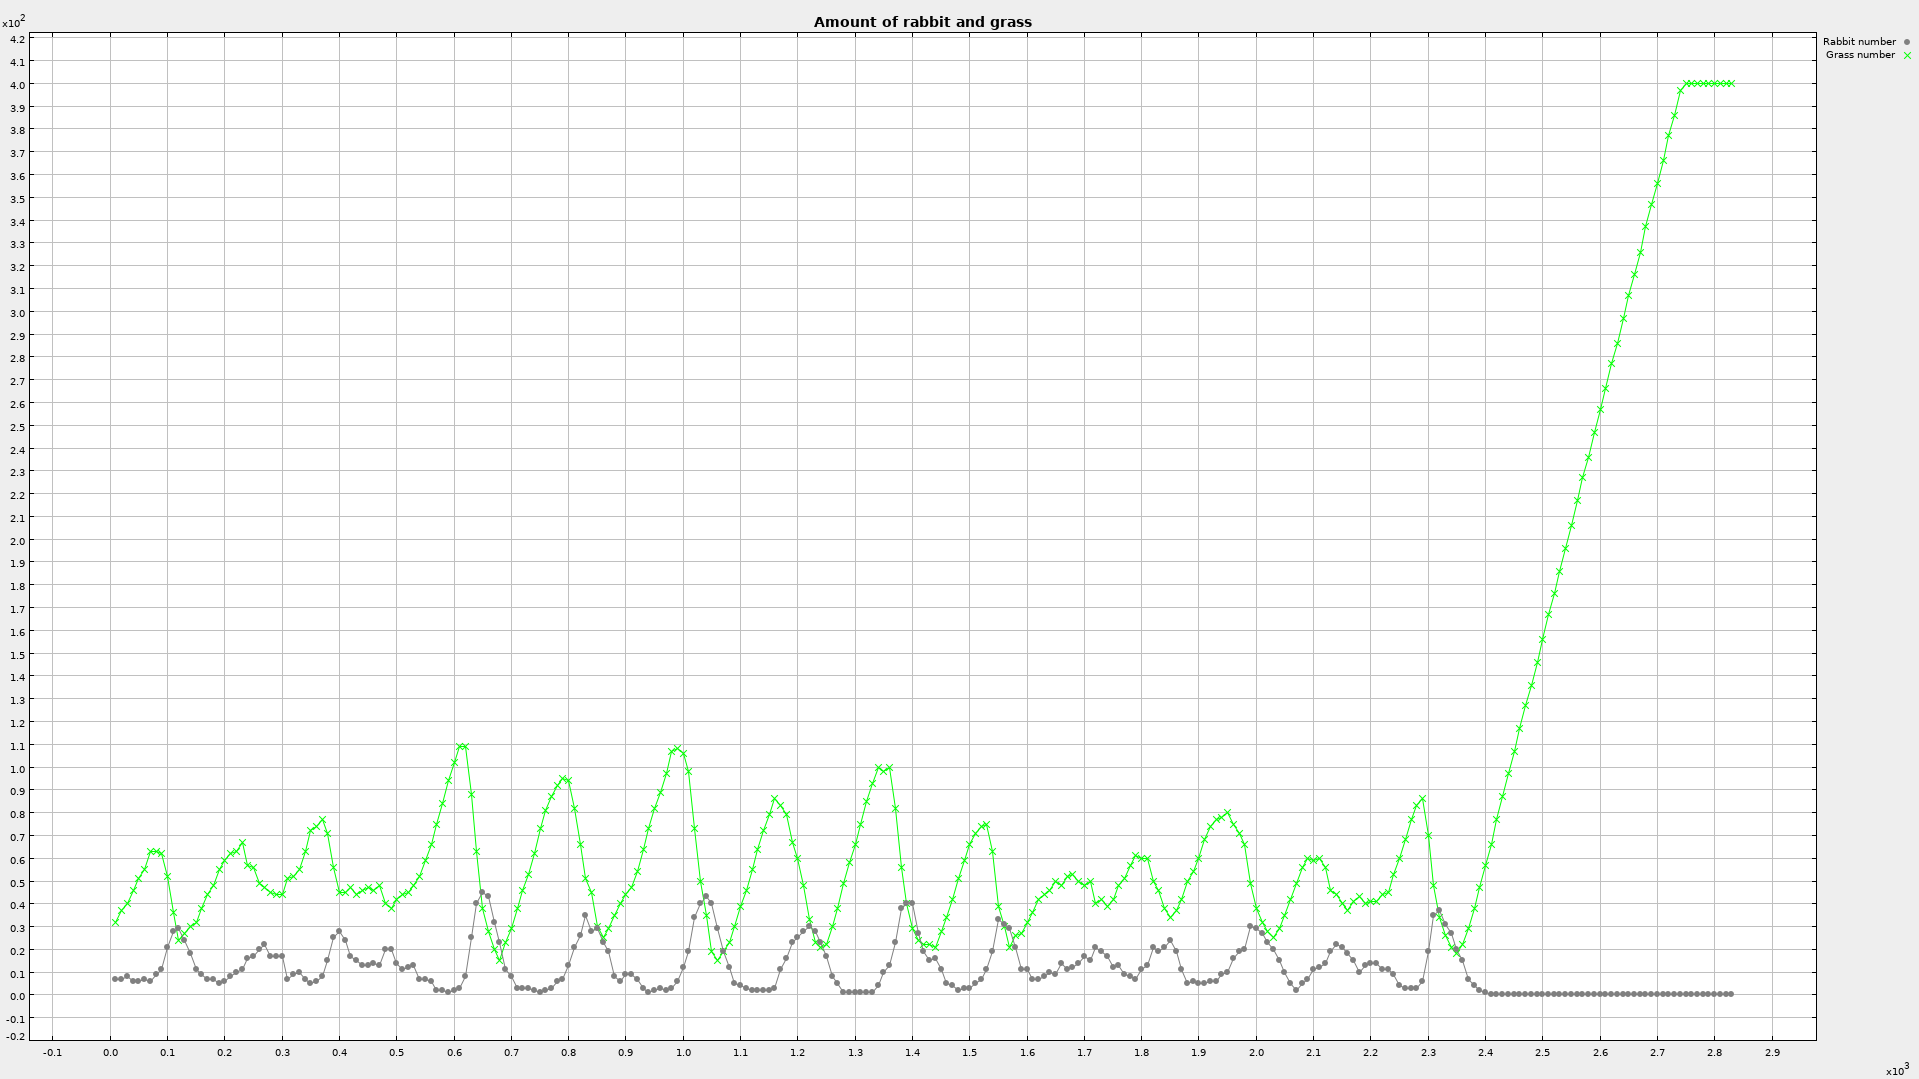
\includegraphics[width=1\linewidth, height=5cm]{setting3_3.png} 
\caption{Population plot for GrassGrowthRate = 1.}
\label{fig:image2}
\end{figure}


\subsection{Experiment 3}

\subsubsection{Setting}
In this final experiment, variations of the BirthThreshold parameter are studied and its effects on the simulation are described.

\subsubsection{Observations}
% Elaborate on the observed results %
The BirthThreshold significantly affects the simulation for high values: when it is lower than 50, the grid is full of rabbits but as soon as we increase the parameter for values higher than 50 we see a more general stability between rabbits and grass units, with rabbits always more than grass units. It is interesting to notice that there's still an equilibrium when the BirthThreshold is equal to 100 (maximum). This is likely due to the high values set for the other parameters. For example, by decreasing EatGrassEnergy to 10, grass units start growing more quickly in the same setting. 


\end{document}